\documentclass[a4paper]{memoir}

%%%%% Packages %%%%%
\usepackage{lmodern}
\usepackage{palatino}
\usepackage[T1]{fontenc}
\usepackage[utf8]{inputenc}

% To be removed if you want it in english
\usepackage[french]{babel}

\usepackage{amstext,amsmath,amssymb,amsfonts}
\usepackage{multirow,colortbl}
\usepackage{xspace,varioref}
\usepackage{hyperref}

\usepackage[dvipsnames]{xcolor}
\usepackage{graphicx}

\usepackage{appendix}
\usepackage{makeidx}

%% custom style %%%%%%%%%%%%%%%%%%%%%%%%%%%%%%%%%%%%%%%%%%%%%%%%%%%%%%%%

% custom commands
\newcommand{\version}[1]{\def\theversion{#1}}
\newcommand{\subtitle}[1]{\def\thesubtitle{#1}}

\newcommand{\authors}[1]{\def\theauthors{#1}\author{#1}}
\newcommand{\supervisor}[1]{\def\thesupervisor{#1}}
\newcommand{\tutor}[1]{\def\thetutor{#1}}

% translation for custom words
\newcommand{\authorname}{Author}
\newcommand{\authorsname}{Authors}
\newcommand{\supervisorname}{Supervisor}
\newcommand{\tutorname}{Tutor}

\newcommand{\thepartname}{Part}

\ifdefined\addto{%
\addto{\captionsfrench}{\renewcommand{\authorname}{Auteur}}%
\addto{\captionsfrench}{\renewcommand{\authorsname}{Auteurs}}%
\addto{\captionsfrench}{\renewcommand{\supervisorname}{Superviseur}}%
\addto{\captionsfrench}{\renewcommand{\tutorname}{Tuteur}}}
\addto{\captionsfrench}{\renewcommand{\thepartname}{Partie}}
\else{}
\fi

%%%%% Setting Titlepage %%%%%
%%%%%%%%%%%%%%%%%%%%%%%%%%%%%
\pretitle{\flushleft\Huge\textsf}
\posttitle{\\[-.65em]\rule{\linewidth}{1.5mm}\\[-.65em]
\ifx\thesubtitle\undefined%
\else%
  \hfill{\small\itshape \thesubtitle}%
\fi
\centering
\vfill

\includegraphics{Universite_de_Bordeaux.pdf}
\vfill
\iflanguage{french}{
{\Huge Projet de deuxième année}
}{
 {\Huge Master2 Project}
}\\
\vspace{1.25em}
\iflanguage{french}{%
  \LARGE
  Master \emph{Sciences et Technologies},\\
  Mention \emph{Informatique},\\
% Mention \emph{Mathématiques},\\
  Parcours \emph{Cryptologie et Sécurité Informatique}.\\
  \par\hfill%
}{%
  \LARGE
  Master in \emph{Sciences and Technologies},\\
  Specialty in \emph{Computer Science},\\
% Specialty in \emph{Mathematics},\\
  Track \emph{Cryptology and Computer Security}.\\
  \par\hfill
}}

%% author
\preauthor{\vspace{\fill}\\
\ifx\theauthors\undefined%
  \flushleft\textbf{\large\authorname}\\
\else%
  \flushleft\textbf{\large\authorsname}\\
\fi
\small}
\postauthor{\vspace{1em}
\ifx\thesupervisor\undefined%
\else%
  \newline\textbf{\large\supervisorname}\\\thesupervisor\\[1em]%
\fi
\rule{\linewidth}{1mm}\\[-.25em]}

%% version and date
\predate{\hspace{\fill}
\ifx\theversion\undefined%
\else%
  version~\theversion~--~%
\fi}
\postdate{}

%% chapters style %%%%%%%%%%%%%%%%%%%%%%%%%%%%%%%%%%%%%%%%%%%%%%%%%%%%%%
%% You may try several styles (see more in the memoir manual).

\chapterstyle{veelo}
%\chapterstyle{chappell}
%\chapterstyle{ell}
%\chapterstyle{ger}
%\chapterstyle{pedersen}
%\chapterstyle{verville}
%\chapterstyle{madsen}
%\chapterstyle{thatcher}

%% parts style %%%%%%%%%%%%%%%%%%%%%%%%%%%%%%%%%%%%%%%%%%%%%%%%%%%%%%%%%

\renewcommand*{\thepart}{\arabic{part}}

\renewcommand*{\parttitlefont}{\chaptitlefont\Huge}
\renewcommand*{\partnamefont}{\chapnamefont\HUGE}
\renewcommand*{\partnumfont}{\chapnumfont\HUGE}

\renewcommand{\beforepartskip}{\vspace*{\fill}}
\renewcommand{\midpartskip}{\vspace{.5em}\hrule height 1.5mm \vspace{.5em}}
\renewcommand{\afterpartskip}{\vspace*{\fill}}

% table of contents
\renewcommand*{\cftpartname}{\thepartname}
\renewcommand*{\cftpartpresnum}{\space}
\renewcommand*{\cftpartaftersnum}{.}
\renewcommand*{\cftpartaftersnumb}{\space}

\cftpagenumbersoff{part}
\renewcommand{\cftpartafterpnum}{\protect\\[-.75em]%
  \protect\mbox{}\protect\hrule\par}

\renewcommand{\cftchapterdotsep}{4}


%% index generation %%%%%%%%%%%%%%%%%%%%%%%%%%%%%%%%%%%%%%%%%%%%%%%%%%%%
\makeindex

%%%%% Useful macros %%%%%
\newcommand{\latinloc}[1]{\ifx\undefined\lncs\relax\emph{#1}\else\textrm{#1}\fi\xspace}
\newcommand{\etc}{\latinloc{etc}}
\newcommand{\eg}{\latinloc{e.g.}}
\newcommand{\ie}{\latinloc{i.e.}}
\newcommand{\st}{\ensuremath{\text{\xspace s.t.\xspace}}}


%%%%% Report Title %%%%%
\title{Attaque sur SSL/TLS}
\subtitle{Poodle et Triple-Handshake RSA}

\authors{Youri Laforgue \texttt{<youri.laforgue@etu.u-bordeaux.fr>}\\
Stewie Suivant \texttt{<stewie.suivant@etu.u-bordeaux.fr>}}

\supervisor{Abdou Guermouche \texttt{abdou.guermouche@labri.fr}}

%\version{0.1}

%%%%% Document %%%%%
%%%%%%%%%%%%%%%%%%%%
\begin{document}

\frontmatter%%%%%%%%%%%%%%%%%%%%%%%%%%%%%%%%%%%%%%%%%%%%%%%%%%%%%%%%%%%%
\maketitle
 \thispagestyle{empty}

 \cleardoublepage
\par\vspace*{\fill}

\iflanguage{french}{%
\section*{Déclaration de paternité du document}
}{%
\section*{Declaration of authorship of the document}}

\ifx\theauthors\undefined%
\iflanguage{french}{%
  Je certifie sur l'honneur que ce document que je soumet pour
  évaluation afin d'obtenir le diplôme de Master en \emph{Sciences et
    Technologies}, Mention \emph{Mathématiques} ou
  \emph{Informatique}, Parcours \emph{Cryptologie et Sécurité
    Informatique}, est entièrement issu de mon propre travail, que
  j'ai porté une attention raisonnable afin de m'assurer que son
  contenu est original, et qu'il n'enfreint pas, à ma connaissance,
  les lois relatives à la propriété intellectuelle, ni ne contient de
  matériel emprunté à d'autres, du moins pas sans qu'il ne soit
  clairement identifié et cité au sein de mon document.
  \bigskip

  \hfill\textbf{Date et Signature}
}{%
  I hereby certify that this material, which I now submit for
  assessment on the programme of study leading to the award of the
  Master in \emph{Sciences and Technologies}, Specialty in
  \emph{Mathematics} or \emph{Computer Science}, Track
  \emph{Cryptology and Computer Security}, is entirely my own work,
  that I have exercised reasonable care to ensure that the work is
  original, and does not to the best of my knowledge breach any law of
  copyright, and has not been taken from the work of others save and
  to the extent that such work has been cited and acknowledged within
  the text of my work.
  \bigskip

  \hfill\textbf{Date and Signature}}
\else%
\iflanguage{french}{%
  Nous certifions sur l'honneur que ce document que nous soumettons
  pour évaluation afin d'obtenir le diplôme de Master en
  \emph{Sciences et Technologies}, Mention \emph{Mathématiques} ou
  \emph{Informatique}, Parcours \emph{Cryptologie et Sécurité
    Informatique}, est entièrement issu de notre propre travail, que
  nous avons porté une attention raisonnable afin de nous assurer que
  son contenu est original, et qu'il n'enfreint pas, à notre
  connaissance, les lois relatives à la propriété intellectuelle, ni
  ne contient de matériel emprunté à d'autres, du moins pas sans qu'il
  ne soit clairement identifié et cité au sein de notre document.
  \bigskip

  \hfill\textbf{Date et Signatures}
}{%
  We hereby certify that this material, which we now submit for
  assessment on the programme of study leading to the award of the
  Master in \emph{Sciences and Technologies}, Specialty in
  \emph{Mathematics} or \emph{Computer Science}, Track
  \emph{Cryptology and Computer Security}, is entirely our own work,
  that we have exercised reasonable care to ensure that the work is
  original, and does not to the best of our knowledge breach any law
  of copyright, and has not been taken from the work of others save
  and to the extent that such work has been cited and acknowledged
  within the text of our work.\bigskip

  \hfill\textbf{Date and Signatures}}
\fi
\vspace{6em}


 \cleardoublepage
\tableofcontents*

\chapter*{Introduction}

\paragraph{}
SSL (Secure Sockets Layer) et TLS (Transport Layer Security) définissent des protocoles 
permettant de sécuriser des échanges sur internet. SSL a été initiallement développé 
par Netscape en 1995, avec la version SSL 2.0. L'IETF prend le relais à la suite de la 
version SSL 3.0, et renomme le protocole TLS. La dernière version à ce jour est 
TLS 1.2 sorti en 2008.

Pour des raison de compatibilité, la majeure partie de ces versions sont 
encore utilisé à l'heure actuel.

\paragraph{}
TLS Fonctionne en mode client-serveur, et permet de répondre à plusieurs objectifs :
\begin{itemize}
\item L'authentification du serveur et/ou du client (authentification mutuelle).
\item La confidentialité des données échangées.
\item L'intégrité des données échangées.
\end{itemize}



\paragraph{}
Son objectif initial et principal est de sécuriser le protocole HTTP, 
notamment pour sécuriser les paiements en ligne lors de l'essort du e-commerce. 
Aujourd'hui, son champs d'application s'est étendu : protection d'autres 
protocoles comme SMTP ou LDAP, création de VPN, etc...

\paragraph{}
Ce protocole étant largement utilisé par les serveurs et navigateurs web 
pour la sécurisation des échanges sur internet, 
il est également la cible de nombreuse attaques visant à voler une connexion, 
usurper une identité, écouter le trafic pour récolter des informations sensibles 
(mot de passe, information bancaire, etc...).

\paragraph{}
Nous allons faire, dans un premier temps, 
le tour des attaques découvertes à partir de 2011, reposant sur différents mécanismes. 
Dans un deuxième temps, nous rentrerons dans le détails de deux attaques récentes, 
à savoir POODLE et 3-Handshake, verrons leur implémentation et aborderons 
les contres-mesures envisageables. 
Nous conclurons en ......................................................... .


\addcontentsline{toc}{chapter}{Introduction}

\mainmatter%%%%%%%%%%%%%%%%%%%%%%%%%%%%%%%%%%%%%%%%%%%%%%%%%%%%%%%%%%%%%
\part{SSL/TLS}

\chapter{Présentation}
\chapter{Avantages/Inconvénients}

%%%%%%%%%%%%%%%%%%%%%%%%%%%%%%%%%%%%%%%%%%%%%%%%%%%%%%%%%%%%%%%%%%%%%%%%
\part{Attaques sur SSL/TLS}

\chapter{Attaques Connues}

\chapter{Présentation}
\label{chapter:poodlePres}

L'attaque Poodle (Padding Oracle On Downgraded Legacy Encryption)

a été découverte par Bodo Möller, Thai Duong et 
Krzysztof Kotowicz\cite{article:ssl-poodle} en septembre 2014.\\

Cette attaque se base sur une faiblesse de SSLv3.
Elle fonctionne pourtant sur les dernières versions de TLS.
Pour maintenir la compatibilité avec tout les clients, un
serveur TLS peut rétrograder en version SSLv3.\\

C'est une attaque de typer Man-In-The-Middle (l'homme du milieu).
L'attaquant peut utiliser un site malveillant qui injecte un
code javascript sur le client pour le faire générer des requêtes
sur le serveur cible. Il peut alors forcer l'utilisation de 
SSLv3, même si le client et le serveur utilisent TLS.\\

L'objectif de l'attaque est de voler le cookie de session 
du client. Pour cela, comme BEAST, l'attaquant force 
l'utilisation du mode CBC. Elle utilise le \emph{padding oracle attack }

\chapter{Padding Oracle Attack}
\label{chapter:POA}

Cette attaque a pour objectif de retrouver le clair d'un bloc chiffré 
avec le mode CBC. Elle s'appuie sur le fait que le dernier bloc chiffré
contient du padding. De plus le dernier octet de padding corespond à la
taille du padding.\\

L'oracle  déchiffre le clair et vérifie que la taille du padding est correcte. 
Il renvoie une erreur en cas de taille erronée.\\

Supposons maintenant que l'attaquant posséde un chiffré composé de 4 blocs :
$C1||C2||C3||C4$. Le bloc $C4$ contient un padding de taille $x$ connu par l'attaquant.
il souhaite connaitre le contenu de $C2$ et quand il interoge l'oracle, celui-ci lui dit
si la taille est correcte ou non.\\
L'attaquant peut envoyer une version contrefaites du chiffré comme suit :
$C1||C2||C3'||C4'$.\\
\begin{itemize}
\item le bloc $C4'=C2$
\item le bloc $C3'= C3$ dont le dernier octet est modifié
\end{itemize}
Soit $Pn$ le déchiffrement de $Cn$ par l'oracle et D() et E() les algorithmes
de déchiffement et de chiffrement. 
Le bloc qui nous intérésse est $P4'$.
\[P4' = D(C2) + C3'\]
or $C2 = E(P2 + C1)$ d'où
\[\Longleftrightarrow P4' = D(E(P2 + C1)) + C3'\]
\[\Longleftrightarrow P4' = P2 + C1 + C3'\]
\begin{itemize}
\item $C1$ et $C3'$ sont connus
\item $P2$ est le clair recherché
\item $P4'$ est inconnu mais l'oracle nous dit si le dernier octet égale à $x$.
\end{itemize}
Soit k la taille des blocs et Pn[i] le iéme octet du bloc n.

\[P4'[k] = P2[k] + C1[k] + C3'[k]\] si $P4'[k] = x$ alors
\[\Longleftrightarrow x = P2[k] + C1[k] + C3'[k]\]
\[\Longleftrightarrow P2[k] = x + C1[k] + C3'[k]\]

Ce qui donne une equation a une seule inconnu donc l'attaquant a trouvé $P2[k]$.
Pour avoir $P4' = x$, il suffit de faire varier la valeur de $C3'[k]$. Il est donc
possible de trouver le dernier octet de $P2$ en maximum de 256 essais.\\

Pour trouver les autres octets, l'attaquant prend $P4'[k] = P2[i]$ où $i \in [1,k]$.
Avec cette méthode il est possible de retrouver tout le contenu d'un chiffré à
l'exeption du premier bloc (sauf si l'IV est connu).

\chapter{Mise en place de l'attaque}
\label{chapter:Poodleattack}



\chapter{Triple-Handshake RSA}
\label{chapter:RSA}

\section{Présentation}
\label{sec:pTHR}

l'attaque\up{\cite{article:handshake}} a été découverte par Antoine Delignat-Lavaud, Karthikeyan Bhargavan et Alfredo Pironti 
de l'équipe de recherche Prosecco de INRIA Paris-Rocquencourt. 

Elle est présenté comme une nouvelle classe d'attaque. Un client se connecte sur un serveur malicieux et le serveur
se connecte sur un serveur cible en se faisant passer pour le client. C'est une attaque MITM sur trois Handshake.
L'attaquant réussit l'attaque s'il réussit à se faire passer pour le client après la troisième poignée de main.


\section{Comment ça marche}
\label{sec:ccmTHR}

L'attaque se passe en trois étapes :

\subsection{Etape 1}
\label{sec:e1}

\begin{figure}[h]
\label{fig:hand1}
\centering
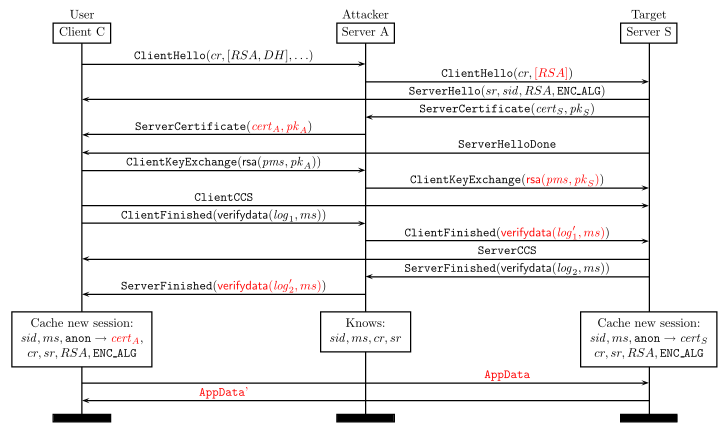
\includegraphics[scale=0.4]{Hand1}
\caption{Triple Handshake : Etape 1}
\end{figure}

Le client $C$ se connecte sur le serveur malicieux $A$. Dans le même temps, $A$ se connecte au serveur $S$ en utilisant
les informations de connexion de $C$. L'attaquant change la requête ClientHello pour imposer le choix de RSA. $A$
doit donner à $C$ et $S$ ses certificats.

$A$ va alors pouvoir récupérer le PMS ( Pre Master Secret ), et le réemettre au serveur. Il doit ensuite modifier
les logs. Ces messages sont les premiers à être chiffré et contiennent un hashé de l'ensemble 
des messages échangés pendant la négociation. Il doit donc les modifiés pour les faire corespondre au log de $C$ et $S$.

L'attaquant a deux connexions avec les mêmes paramètres et clés mais avec des certificats serveur et des logs 
différents. La première poignée de main est finie.

\subsection{Etape 2}
\label{sec:e2}

\begin{figure}[h]
\label{fig:hand2}
\centering
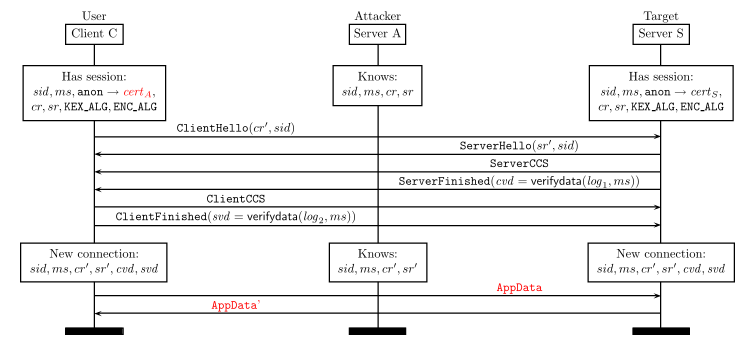
\includegraphics[scale=0.5]{Hand2}
\caption{Triple Handshake : Etape 2}
\end{figure}

$C$ se reconnecte à $A$ et demande un résumé de la connexion précédente. $A$ se reconnecte en retour à $S$ et demande la même chose.
Ensuite $A$ va seulement retransmettre les messages de $C$ vers $S$ et inversement.

A la fin de cette deuxième poignée de main, $C$ et $S$ ont maintenant les mêmes logs. Ils ont aussi négocier de
nouvelles clés, mais comme $A$ est au milieu, il les connait. 
\pagebreak

\subsection{Etape 3}
\label{sec:e3}

\begin{figure}[h]
\label{fig:hand3}
\centering
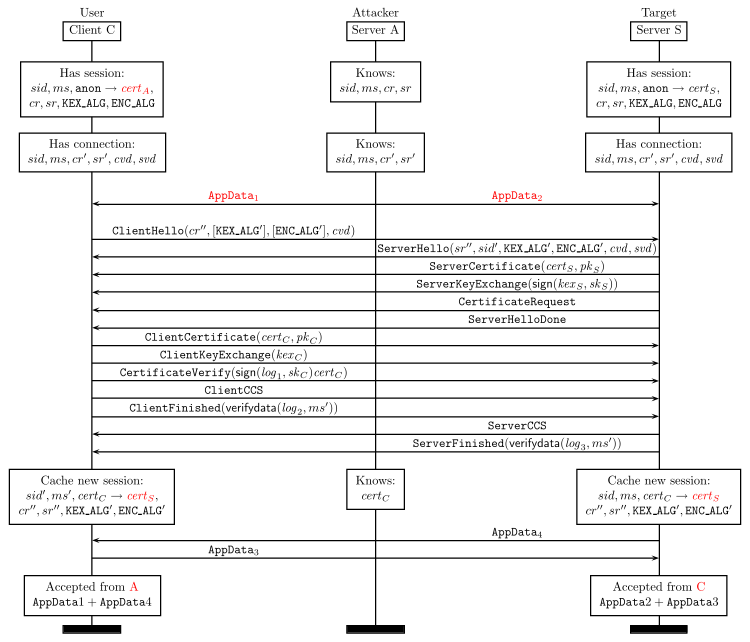
\includegraphics[scale=0.4]{Hand3}
\caption{Triple Handshake : Etape 3 }
\end{figure}

$S$ demande la renégociation complète avec authentification à $A$, qui envoi la demande à $C$. $A$ va seulement faire suivre les messages. A la
fin de la rénégociation, les données de connexion de $C$ et $S$ sont les mêmes. $S$ va envoyer son certificat à $C$.
En principe, $C$ devrait rejetter ce certificat mais en réalité il est accepté par de nombreux navigateurs. La raison
est simple, un serveur peut changer de certificat, parce qu'il a expiré par exemple.

Toutefois, $A$ n'a plus connaissance de la clé de session ou de la nouvelle master key. En effet, pour evoyer
le master secret, $C$ a utilisé la clé publique du certificat de $S$ donc $A$ ne peut pas la déchiffrer.
 Il ne peut donc pas agir ou observer les communications entre le client et le serveur. 

Cette vulnérabilité n'est pas exploitable seule. Cependant, $A$ peut par exemple retransmettre l'image exacte du site de $S$ en
y intégrant un script qui permet d'utiliser une attaque outrepassant le SOP.


\section{Contre-Mesures}
\label{sec:cmTHR}

Pour éviter ces attaques, il faudrait revoir la politique de TLS vis à vis du changement des certificats.
Il faudrait interdire de changer les certificats durant une renégociation. Ainsi la troisième étape ne 
fonctionnerait plus.

Une autre possibilité est de rajouter au master secret un hash du précédent handshake. Ainsi lors d'une
renégociation, le client et le serveur peuvent vérifier leur intégrité respective. Dans notre attaque, 
le hash sera éronné puisque $C$ aura l'identité de $A$ au lieu de $S$, de même pour $S$.

 



%%%%%%%%%%%%%%%%%%%%%%%%%%%%%%%%%%%%%%%%%%%%%%%%%%%%%%%%%%%%%%%%%%%%%%%%

\chapter*{Conclusion}
\label{chapter:ccl}

SSL s'est plein de failles donc c'est \textbf{NUL}.


%%%%%%%%%%%%%%%%%%%%%%%%%%%%%%%%%%%%%%%%%%%%%%%%%%%%%%%%%%%%%%%%%%%%%%%%

\part*{Annexes}
\addcontentsline{toc}{part}{Annexes}
\appendix

\backmatter%%%%%%%%%%%%%%%%%%%%%%%%%%%%%%%%%%%%%%%%%%%%%%%%%%%%%%%%%%%%%

\nocite{*}
\bibliographystyle{plain}
\bibliography{bibliography}

\printindex

\end{document}
